\documentclass[11pt,letterpaper]{article}
\usepackage[margin=1in]{geometry}
\usepackage[english]{babel}
\usepackage[utf8x]{inputenc}
\usepackage{amsmath}
\usepackage{amssymb} 
\usepackage[retainorgcmds]{IEEEtrantools}
\usepackage{graphicx}
\usepackage{tabularx}
\usepackage{epstopdf}
\usepackage{subfig}
\usepackage{bbm}
\usepackage{kpfonts}    % for nice fonts
\usepackage{microtype} 
\usepackage{booktabs}   % for nice tables
\usepackage{bm}         % for bold math
\usepackage{listings}   % for inserting code
\usepackage{verbatim}   % useful for program listings
\usepackage{color}  
\usepackage[colorlinks=true]{hyperref}
\usepackage{setspace}
% use for hypertext
\usepackage[colorinlistoftodos]{todonotes}
\usepackage{natbib}
\usepackage{authblk}
\usepackage[hang,flushmargin]{footmisc} %dont indent footnotes
\newcommand{\hilight}[1]{\colorbox{yellow}{#1}}
\hypersetup{colorlinks=true,linkcolor=black,citecolor=black,urlcolor=black}

\newcolumntype{K}[1]{>{\centering\arraybackslash}p{#1}}



\title{The Effect of Local Labor Market Downturns on Postsecondary Enrollment and Program Choice\thanks{ Foote: Center for Economic Studies, U.S. Census Bureau, andrew.foote@census.gov. Grosz: Department of Economics, University of California Davis, mgrosz@ucdavis.edu. Special thanks to Massimo Anelli,  Dave Carlson and Matt Naven. Any opinions and conclusions expressed herein are those of the author(s) and do not necessarily represent the views of the U.S. Census Bureau. All results have been reviewed to ensure that no confidential information is disclosed.}}

\date{\today\\  }



\author[1]{Andrew Foote} 
\author[2]{Michel Grosz}
\affil[1]{Center for Economic Studies, U.S. Census Bureau}
\affil[2]{Department of Economics, University of California, Davis}


\begin{document}

\begin{abstract}

We examine how workers invest in human capital following job displacements. We make two key contributions considering prior work on this topic. First, we focus on local labor market shocks, using counts of workers involved in localized mass layoff events over the past two decades.  We find that, on average, two-year college enrollment increases by three students within three years for every 100 workers laid off. Second, we show that in addition to enrollment effects, there are heterogenous completion responses by field of study. The largest responses are in high-return fields, though this relationship is likely limited by institutional constraints.

\end{abstract}


\doublespacing
\clearpage 

\section{Introduction}
 The dynamics of worker adjustment following job loss have gained renewed interest in light of the recent Great Recession and  declines in labor force participation \citep{wh2016}. Some workers  regain employment quickly, but many exit the  labor force. However, it remains an open question what workers do upon exiting the labor force, especially as they take an increasingly long time to re-enter the ranks of the employed.\footnote{In previous work, we have considered cross-county migration flows, enrollment in public benefit programs, and non-participation \citep{FGS2015}.} Workers who exit the labor force may experience significant depreciation in human capital, which has permanent productivity and wage consequences \citep{AES1999,GdG2009}. However, some workers exit the labor force to upgrade their skills.  Thus, it is crucial to understand to what extent workers enter postsecondary institutions in bad economic times, as well as what fields they study.
 
There is considerable research documenting the relationship between job loss and postsecondary enrollment. However, the literature tends to measure either individual responses to personal job loss \citep[e.g.][]{BT2015} or aggregate effects of large macroeconomic shocks \citep[e.g.][]{BD2012}. Much less is known about the effect at the local labor market level, where the contraction of specific industries or downsizing of large employers may have outsized ripple effects. It is particularly important to understand these dynamics across the entire local labor market since some workers not directly affected by job loss may also respond to an adverse economic climate by enrolling in school.

In this paper, we consider postsecondary education as a channel for worker adjustment following local economic shocks. Community colleges are the primary engines of worker retraining, especially for older and non-traditional students. Because these are the workers who are most likely affected by local economic downturns, understanding the role of community colleges in the adjustment of local labor markets is particularly important. We consider  enrollment outcomes as well as the receipt of degrees and certificates, and we distinguish between two-year associate's degrees and other certificates and diplomas. Additionally, we group awards by field of study and duration, focusing in particular on how degree completion in career-technical education fields responds to labor market shocks. We also pay close attention to fields with rapidly rising or declining labor demand, such as  health, information technology, and manufacturing. 

This paper makes several contributions to the literature. In contrast to previous papers in the literature, we use mass layoffs as a  measure of adverse labor demand changes. Mass layoffs are  a large, acute shock to employment for workers, and not open to many of the methodological limitations common to studies of this kind.\footnote{As we outline in a later section, many similar studies use the unemployment rate as the measure of local demand shocks. This has several drawbacks, not least of which is the endogeneity of the unemployment rate to exits from the labor force such as educational enrollment.} Second, our analysis  spans the entire country, while other papers have considered  specific industries, areas, or workers. Third, we focus primarily on the effects at the two-year college level, in the spirit of the influential  analysis by \citet{BF1995}. While we replicate their finding on the counter-cyclicality of enrollment with respect to local labor demand shocks, we also separately estimate effects for completion in different types of degree and certificate programs. Finally, our data allow us to test for differences in response during the Great Recession, when labor  demand shocks were particularly acute. 

We find that following mass layoff events, there is a marked increase in community college enrollment. Our main results suggest that for every 100 workers laid off, enrollment increases by three students within the next three years. This enrollment channel accounts for approximately half of the size of the labor force non-participation following mass layoff events, which we document in \citet{FGS2015}. Additionally, we find that for 100 workers involved in a mass layoff, approximately two workers end up receiving a degree or certificate. When we examine different types of awards separately, we find that the bulk of this effect is concentrated among certificates, as opposed to associate's degree programs. 

We also find that there is heterogeneity in the extent to which workers complete different programs following layoff events. There are much larger responses in career-technical fields than in academic fields focused on transfer to four-year colleges. Within career-technical fields, we find particularly large effects for associate's degrees in construction and manufacturing, as well as certificate programs in allied health.\footnote{Examples of allied health programs include medical and nursing assistants, dental hygienists and assistants, emergency medical technicians, and radiologic technologists.} Overall, we find a positive though weak correlation between a particular program's completion response to layoff events and its estimated earnings return, which we take as suggestive evidence that workers leaving the labor force to retrain enroll in high-return fields. 

%In future work, we also want to look at how TAA and WIA funding levels increase or dampen these enrollment and receipt effects, and how this differs based on the size of geographic location of the area where the layoff took place.

The remainder of this paper proceeds as follows. Section \ref{sec:literature} reviews the previous literature on the topic, and Section \ref{sec:data} discusses our data. To motivate our analysis, Section \ref{sec:edllm} presents aggregate trends in postsecondary enrollment and degree receipt, as well as the geographic variation in postsecondary enrollment. Section \ref{sec:meth} outlines our research design, while Section \ref{sec:results} presents our results. Section \ref{sec:conclusion} concludes and discusses potential directions for future work.

\section{Literature \label{sec:literature}}
A large literature has shown the adverse effects of job loss on workers. \citet{JLS1993} show that workers involved in a mass layoff lose about 25 percent of their earnings over the next six years. Additionally, \citet{Stevens1997} shows that much of this effect can be explained by  individuals losing subsequent jobs, effectively compounding the adverse effects. However, recent literature has shown that while the mean effect of job loss is quite negative, the dispersion of outcomes for displaced workers is large; \citet{FHM2012} find that a worker at the 10th percentile of outcomes experiences a 10 percent decline in earnings, while a worker at the 90th percentile sees a 14 percent increase in earnings following a mass layoff. These results suggest that some workers actually benefit from being laid off, and one potential channel to explain this earnings growth is increased human capital accumulation following the separation.

There is also a growing literature documenting worker labor force exit following adverse labor demand shocks. \citet{ADH2013} show that workers in areas experiencing lower labor demand because of increased trade competition drop out of the labor force at higher rates than workers in areas not exposed to this competition. \citet{FGS2015} find that following a mass layoff, about half of the adjustment in labor force size is due to non-participation, but what workers do upon exit is not examined.  \citet{Yagan2016} also shows that non-participation is particularly important in the Great Recession.

In addition to findings on worker displacement, there is strong evidence that postsecondary enrollments are counter-cyclical. \citet{BF1995} find that unemployment rate increases of one percentage point lead to enrollment increases of four percentage points, and similar recent work uses similar designs \citep{HO2013, Nutting2008, clark2011}. Additionally, recent evidence shows that enrollment in the two-year and four-year sectors increased considerably due to the Great Recession \citep{BD2012}, but there is much less evidence on whether the content of what people study is affected by downturns. An exception is \citet{Nutting2008}, who finds that career technical enrollment is more responsive to labor market conditions than academic enrollment at one large public university.\footnote{A growing number of papers using natural experiments focus on educational impacts of natural resource booms \citep{Basso2016, BMS2005, MCL2015,CN2015},\footnote{\citet{Basso2016} also examines the effect of the bust following an oil boom.} though most consider the high school dropout margin as opposed to the college enrollment decision.}

Recent work  also examines the skill upgrading of displaced workers. \citet{BT2015} find that longer unemployment insurance duration and more generous unemployment insurance policies increase the likelihood of individuals to enroll in postsecondary education. \citet{JLS2005b, JLS2005a} use administrative data from Washington and find that workers who enroll in schooling following a job loss have increased earnings, even for older workers. 

There is also growing interest in how postsecondary institutions themselves act as economic agents, and whether they respond to local changes in labor demand. This interest is partially related to the rise of  two-year for-profit colleges, leading to concern about competition between the public and the private sector \citep{DGK2012, Cellini2009, Cellini2010}. \citet{Xia2016} shows that for-profit schools compete with community colleges over specific programmatic offerings, though on the whole they seem more responsive to incentives from financial aid availability than the local demand for skills \citep{Cellini2010b}. \citet{Xia2016} also finds that community colleges are rigid in their course offerings and class  sizes.


\section{Data \label{sec:data}}
his section outlines the main data sources that we use for the analysis. While all the data we collect is reported at the county or sub-county level, we aggregate the data to the commuting zone level \citep{TS1996}. Commuting zones 
approximate the boundaries of a local economy according to commuting patterns, thus reducing the likelihood of confounding spillovers due to local migration and commuting. Moreover, because commuting zones are aggregations of counties, they are straightforward to use with publicly provided data. In our context, the use of commuting zones is useful for two other reasons. First, students are not constrained to attend community college in their county. Furthermore, many counties do not have any postsecondary institutions, meaning that we would need to drop them from the analysis, and thus lose a considerable segment of potential college enrollees. On the other hand, we believe that states are too large a definition of a local labor market, especially since two- and four-year colleges tend to draw students locally.\footnote{\citet{BL2009} find that, in Ohio, the median distance between home and four-year college was 26 miles, and over half of students lived within 50 miles.} 

\subsection{Mass Layoffs}
We use mass layoff events as our key measure of local labor market downturns, measured at the county level, which we aggregate to the commuting zone level. Between 1996 and 2013, the Bureau of Labor Statistics (BLS) compiled monthly reports on layoffs by observing the initial claims for unemployment insurance filed by workers. The BLS identified a mass layoff event when more than 50 workers filed claims against a single establishment within a five-week period. For these events, the BLS contacted the establishment to determine whether these workers experienced a layoff of at least 31 days. We use these data to quantify the size of a local labor demand shock at the county level. The data are reported by county of residence and so, for each county, we measure the number of workers residing in that county that were involved in a mass layoff in a given year. 

In other work, we have shown that mass layoffs are a viable measure of local labor market shocks \citep{FGS2015}. Most importantly, they measure a clear change in labor demand, and thus are not hampered by endogenous labor supply responses. Mass layoffs do not represent all instances of job separations for workers, only separations that resulted in 50 or more unemployment insurance claimants. Still, mass layoffs are a good measure in our setting precisely because they account for workers who lose their job, do not find work, and apply for unemployment benefits.\footnote{Unemployment benefits are usually not allowed for students. Nevertheless, unemployed workers may forgo unemployment insurance to enter training programs and community colleges.}  Thus, the number of workers involved in mass layoffs represent a group for whom job re-training is potentially the most advantageous.

In interpreting the estimates that follow, it is important to keep in mind the composition of workers who are represented by mass layoffs. \citet{Handwerker2012} look explicitly at the firms involved in mass layoffs, and note that the workers represented tend to be older and more concentrated in manufacturing and other heavily unionized industries, since this increases the likelihood that, conditional on being laid off, a worker claims unemployment benefits.

\subsection{Education Data}
Our data on enrollment and degree receipt come from the Integrated Postsecondary Education Data System (IPEDS), from the U.S. Department of Education. IPEDS data includes extensive information for all institutions of higher education that participate in federal financial aid programs, as well as some that may volunteer their own data. We focus on two measures of enrollment. These include overall and first-time fall enrollment counts, broken out by gender. 

The data in IPEDS also include information on awards, both degrees and certificates. We focus on  associate's degrees (AA and AS), and two types of certificates: one-to-four year certificates and certificates requiring less than a year.\footnote{There is also information on bachelor's degrees and graduate degrees, but these are not relevant to the margin we are studying. Bachelor's degrees at community colleges are a small and relatively new phenomenon.} We examine degrees and certificates in the aggregate and by broad field of study.\footnote{All awards are categorized by their Classification of Instructional Program (CIP) codes maintained by the U.S. Department of Education National Center for Education Statistics (NCES) and updated periodically. There are over 1,300 CIP codes. To simplify matters, we group them into broader categories. Appendix Table \ref{tab:cipapp} shows the grouping of CIP codes we use.} To further simplify, we categorize certain fields of study as ``career-technical,'' based on a system established by the California Community Colleges \citep{CCCCOtop} and used for external reporting purposes. IPEDS data also provide address data for every year for all institutions. We match each institution with its county and, thus, the number of layoffs in the local area.

Other work has discussed the drawbacks of using the IPEDS to measure the activity of for-profit sub-baccalaureate institutions \citep{Cellini2005, Cellini2010}. In particular, IPEDS tends to undercount these institutions, and is not always accurate in determining their location, which is crucial for our analysis. Nevertheless, we present results including for-profit colleges for our main analyses, with the caveat that they may be subject to  measurement error. 


\subsection{Other Data}
We supplement these main sources of data with additional information on county demographics. We use age, gender, and racial composition information from the Surveillance, Epidemiology, and End Results (SEER) program of the National Cancer Institute. We also use the SEER data to calculate the size of the working age population (ages 16-65). Additionally, we use the Local Area Unemployment Statistics (LAUS) from the BLS in order to measure the size of the labor force and the unemployment rate in the county. 

\section{Descriptive Evidence label{sec:edllm}}

\subsection{Trends in Post-Secondary Enrollment and Degree Receipt }

To better understand how college enrollment responds to macroeconomic conditions, and how college-going rates vary geographically, in this section we present enrollment trends over our study period, with a particular emphasis on the dynamics of the community college sector.



Figure \ref{fig:grenr} shows enrollment from 1996 to 2011, disaggregated by type of institution (4-year, 2-year public and 2-year private). Panel (a) of Figure \ref{fig:grenr} shows fall enrollment counts, while panel (b) shows first-time fall enrollment (i.e. newly enrolled students). In the two most recent recessions, shown as shaded bars, 2-year public enrollment increased markedly, particularly in the most recent recession. In contrast, 4-year enrollment has been secularly increasing since the beginning of our period, with no real changes in the trend in response to business cycles. Also,  while 2-year for-profit schools have received increasing scrutiny, they make up a small portion of enrollment in IPEDS.\footnote{IPEDS does not cover the for-profit sector nearly as well, as noted in Section \ref{sec:data}.}

Figure \ref{fig:grenr} also shows similar trends for degrees and certificates awarded. While there are larger enrollment counts at 4-year schools, panel (c)  shows that associate's degrees are consistently a larger share of total degree receipts, and therefore an important part of the postsecondary education sector. To get a better sense of the composition of 2-year degrees, panel (d) disaggregates the 2-year degrees into field of study, as a share of total degrees conferred. Career-technical education is a large share of total degrees, accounting for almost 60 percent of the degrees in this time period. Additionally, health has been increasing as a share of degrees, while construction and manufacturing degrees have become  less prevalent.

There are also regional differences in postsecondary and community college enrollment, as shown in the maps in Figure \ref{fig:mapenr}, which display the postsecondary enrollment by commuting zone.\footnote{As with our empirical estimates, we choose to display statistics at the commuting zone level, because many counties have no postsecondary institutions, and individuals could easily attend a school in an adjacent county.} Panel (a) of Figure \ref{fig:mapenr} shows enrollment as a share of population in the CZ, and panel (b) shows community college enrollment as a share of total enrollment.  While there is some geographic variation in enrollment in postsecondary, the variation in community college share is particularly striking. Because some areas only have access to community colleges, it is unlikely that workers who are upgrading their skills following a job loss will relocate for schooling. In fact, the strong correlation between community college enrollment and distance to the nearest institution is an often-used instrument for enrollment patterns in this literature \citep{rouse1995, XJ2013,LK2009}.

There are also significant geographic differences in field of study. Figure \ref{fig:mapawa} displays the share of overall community college awards in each field of study. While career-technical education is concentrated in the Rust Belt, there is regional variation in the particular types of programs. For example, childcare and cosmetology are concentrated in the South and in Southern California. On the other hand, health programs are much more broadly represented.

Overall, it is clear that community college enrollment is correlated with macroeconomic labor market conditions, and that career-technical education is an important piece of this response. In addition, there is a considerable amount of regional differences in educational access, enrollment, and attainment in the cross-section as well. We harness both of these levels of variation to estimate the causal effect of local economic shocks on two-year college enrollment and receipt of degrees and certificates. 



\subsection{Sample Summary Statistics}
Table \ref{tab:sumstats} displays summary statistics for the main variables we use for the analysis, for the years 1996-2013, at the commuting zone level. On average, almost 1,500 workers per year were laid off in mass layoff events in each commuting  zone. This represented around 0.6 percent of the labor force each year. In each year approximately a fifth of commuting zones had layoffs of over one percent of the labor force, while two percent of commuting zones had particularly large shocks of over five percent of the labor force laid off. 

Commuting zones have an average of between two and three community colleges, and around twice as many for-profit, two-year schools. Although there were more for-profit than public two year colleges, community colleges represented the lion's share of two-year college enrollment. 


A number of commuting zones had no community colleges or for-profit two-year colleges; these commuting zones are almost exclusively in rural areas, while in a large share of commuting zones---37 percent---two-year colleges represented the only type of postsecondary institution. Given that laid-off workers likely seek to retrain closer to home, this fact provides further motivation for focusing on the community college sector, which primarily draws students from nearby \citep{rouse1995}. 

The last rows of Table \ref{tab:sumstats} show the distribution of the content of degrees and certificates. Forty percent of awards were in career-technical fields. Of these, a quarter were in construction and manufacturing fields. An even larger share of awards were in health fields such as nursing, medical assisting, and various medical technologies such as radiology or respiratory care therapy. Only three percent of awards were in information technology. 


\section{Methodology \label{sec:meth}}


Our goal is to measure the effect of local economic shocks on educational decisions of individuals. To avoid issues of endogeneity and measurement error inherent in using the unemployment rate, we use  mass layoff counts as a measure of local labor demand shocks.\footnote{We discuss the drawbacks of regressing local outcomes on the unemployment rate in more detail in Appendix \ref{sec:appunemp}. For completeness,  Appendix \ref{sec:appunemp} also shows results using this approach.}  Mass layoffs measure acute local shocks to the labor demand, with fewer concerns about measurement error inherent in small area estimation. Moreover, mass layoffs are of independent interest as a concrete measure of the number of jobs lost in a particular type of displacement.\footnote{A commonly used instrument for the unemployment rate to isolate labor demand shocks is the shift-share or ``Bartik'' instrument \citep{SW2011, BH2000}, which leverage pre-existing area-specific industry structure and changes in industry outcomes at the national level. There are a number of reasons why such a method is likely inadequate in the context we study. First, these insstruments do not usually give intuition on the  size of a shock relative to the local labor force. More importantly, the shift-share instruments are better suited to identifying long-run structural shocks, as opposed to the transitory, acute impact of layoffs that we study in this paper. Moreover, as we discuss in \citet{FGS2015}, Bartik demand measures combine local industry structure with trends in national product and labor demand. Education may respond to both local and national business cycle conditions, but here we focus on local measures, so it is not desirable to combine local and national conditions  in a single measure. }

We estimate the effect of a large mass layoff event on enrollment in postsecondary education. In particular, we estimate an elasticity, and allow mass layoffs to impact enrollment in more than one period, since it takes workers time to adjust. To do so, we estimate the following equation:

\begin{equation}\label{eqn:main}
y_{ct} = \sum_{i=1}^I \beta_i m_{c,t-i} + \Theta X_{ct} + \gamma_c + \eta_t +\xi_c*t+ \epsilon_{ct}
\end{equation}

Where $y_{ct}$ is the one of our outcomes of interest, either enrollment or awards, while $m_{ct}$ is the log of the number of workers directly affected by mass layoff events in commuting zone $c$ in year $t$.\footnote{We use commuting zones as our geographic unit of observation because a worker is likely to commute to school within this area.} Since both the outcome and the key regressor are expressed as logs, our estimate of $\beta_i$ can be interpreted as an elasticity.

In the matrix $X_{ct}$ we include a set of time-varying measures of local characteristics. We include commuting zone fixed effects, $\gamma_c$, to account for systematic, time-invariant differences between commuting zones, and  year fixed effects, $\eta_t$, to control for national trends.  All regressions are weighted by the local labor market's lagged total population. Finally, to address the fact that mass layoffs may be correlated within a commuting zone over time, we cluster our standard errors at the commuting zone level.

A crucial element of our main estimating equation is the inclusion of market-specific linear trends $\xi_c*t$. These labor market specific trends  effectively identify the key coefficient $\beta_i$ off deviations from those trends. It is important to account for these trends for a number of reasons. First, we want to control for long-run economic conditions which may also be correlated with funding of community colleges, and other local policies. Second, the demographic composition of certain areas may be changing  over our time period, making the area's population increasingly more or less likely to attend postsecondary institutions. Not controlling for these differential demographic changes would  confound the effect of mass layoffs with demographic changes. Finally, because mass layoffs are concentrated in certain areas of the country, including commuting zone-level trends  identifies the effect off shocks that are deviations from the common trend, as opposed to large shocks per se.\footnote{As an example, consider a commuting zone in which labor demand is decreasing over time, and so there are an increasing number of layoffs every year. Including local trends acknowledges this commuting-zone-specific growth, and the identification comes from layoff events that depart from the trend.}  Given the importance of including local trends, we include them in all our analyses, and present results without linear trends in Appendix Table \ref{tab:firstmain}.

One potential limitation of our approach is that we estimate equation \ref{eqn:main} at an aggregate level, as opposed to using individual-level data on job loss. Thus we are unable to assert that the workers losing their jobs are exactly the individuals enrolling in postsecondary institutions: it may be the case that other workers are responding to slack labor market conditions and choosing to enroll in school. Additionally, there is a possibility that some students are affected because their parents lost their jobs, and choose to enroll in community college as a less expensive alternative to a four-year college \citep{hilger2014}. For this to be a large portion of the effect, we would expect a commensurate decline in four-year school enrollment. We do not find such an effect when estimating equation \ref{eqn:main}, which limits our concern about this issue.

As shown in much of the prior literature, there is a dramatic migration response to local economic downturns \citep{blanchard1992regional}. While we do not explicitly estimate it here, in related work we find a migration response to mass layoffs as well \citep{FGS2015}. If some students are being induced to move across labor markets following economic shocks, this will reduce our estimates of $\beta_i$. In that sense, our estimates are a lower bound for the the effect of mass layoffs on the educational enrollment of students who remain in the labor market.  

\section{Results \label{sec:results}}

\subsection{Enrollment and Completions}

Table \ref{tab:main} shows  results for the main outcomes. The top panel shows results for community colleges and the lower panel shows the same specifications for for-profit colleges. The first column shows that a one percent increase in the number of workers laid off leads to a 0.015 percent increase in community college enrollment, with a smaller effect in subsequent years. The second column displays fall enrollment just among first-time students. We expect this response to be more pronounced than for overall enrollment, because overall enrollment includes continuing students. Indeed, the estimates in the second column of the table are slightly larger than the first column, although the difference is not statistically significant. 

The second panel of the table suggests that for-profit institutions also see positive enrollment effects of a similar magnitude. However, the results are smaller than for community colleges and not statistically significant. While the for-profit sector is a fraction of the size of the public sector, and is likely underrepresented in the IPEDS data, this is still suggestive evidence of a response. However, we certainly do not find any evidence that for-profit enrollments are responding in an outsize way relative to community colleges.

The next four columns of Table \ref{tab:main} explore the effect of layoff shocks on degree receipt. We expect the measured effects to be more muted than for enrollment, because of high attrition rates in the two-year sector, as well as the lag between enrollment and degree completion \citep{CBJK2008}. Still, the third column shows that degree and certificate receipt does respond to layoffs. A one percent increase in layoffs results in a 0.017 percent increase in community college awards two years later, and a 0.004 percent increase three years later. There is a smaller effect at the for-profit level.  Perhaps not surprisingly, the larger effect are for smaller certificate programs that take less time to complete, and also have fewer general education requirements than associate degree programs. 

The timing of the award response is not immediate. At the community college level, the timing is consistent with the length of time required to finish these programs. For example, the effect on the completion of associate's degrees, which take approximately two years of full-time study, is concentrated in the two-year lag, although not statistically significant. Completion of certificates is evenly distributed across all years. 


At the for-profit level, the results are much less precise. There is not a significant increase in associate's degrees following layoffs, as the bulk of for-profit awards are concentrated among shorter-term certificates. We find a large and statistically significant response for certificates only in the third lag. We find large responses for very short certificates at the second and third lags. In general, the main results for for-profit colleges are intuitive. However, given our lack of precision in these estimates, as well as restraint in the general literature on relying too much on for-profit college statistics in the IPEDS data, we focus on community colleges for the remainder of the paper. 

The main result from Table \ref{tab:main} is that there is a positive and statistically significant effect of mass layoffs on enrollment and completion in community colleges. To scale these effects, consider a commuting zone at the mean of the mass layoffs distribution. For 100 workers involved in a mass layoff in this commuting zone, our estimates suggest that first-time enrollment increases by approximately 2.8 students within three years. Moreover, eventual degree receipt increases by 1.9 students over the same period. 

In related work using a similar methodology, sample, and time period, we find that a one percentage point increase in the share of the labor force laid off leads to a 0.2 percentage point decrease in the size of the labor force, of which only half can be explained through observable channels such as migration, retirement, and enrollment in disability insurance \citep{FGS2015}. Our results on enrollment suggest that about half the workers exiting the labor force not through these channels are accounted for by increases in community college enrollment. 


%%%%%%%%%%%%%%%%%%%%%%%%%%%%%%%%%%%%%%%%%%%%%%%%%%%%%%%
\subsection{Field of Study}
Next we estimate the differential responses for degree and certificate production by field of study. Ideally, we would be able to observe enrollment in different types of degree and certificate programs. Identifying which student is enrolled in a particular program, though, is particularly difficult \citep{BSZ2015}. We can only observe completion by program of study, which incorporates a certain measure of endogenous differences in completion rates. Nevertheless, in all cases we expect our estimates of the effect of mass layoffs on program-level completions to be an underestimate, both in terms of the absolute magnitude as well as in the speed of response. Thus, we believe measuring completion can shed light on how workers are responding to displacement.

The first column of Table \ref{tab:mainbyprog} shows the aggregate award response, by type of award. These awards encompass career-technical programs as well as academic programs for students aiming to transfer. In the second column we observe the response just for career-technical programs. Not surprisingly, the results are stronger for CTE awards at all levels, given that displaced workers are likely to enroll in these programs in order to upgrade their skills. 

Columns 3-7 further disaggregate the career-technical awards by the specific content of the programs. We find a large and statistically significant increase in the production of awards in construction and manufacturing fields following layoffs, especially for associate's degrees. This is perhaps surprising given the contemporaneous decline of manufacturing. However, there are a few potential explanations. First, workers laid off in mass layoff events are more likely to be in manufacturing and production fields,  making them also more likely to retrain in manufacturing fields. Second, aggregating all programs of this type ignores the fact that much of the response may be in certain high-growth areas. In fact, in recent years funding from large federal programs such as Trade Adjustment Assistance (TAA) and the Workforce Investment and Opportunity Act (WIA) has gone specifically to high-tech manufacturing programs \citep{wioa2014, eyster2017taaccct}. We return to this issue in the next subsection.

The fourth column of the table examines health programs, which shows a large and statistically significant effect on degree receipt in health programs. In particular, we find the strongest effects for short-term certificates, as opposed to associate's degrees or even long-term certificates. Small certificates grow almost 0.06 percent in the first year following a one percent increase in layoffs. These small certificates are generally for medical assisting, nursing assisting, and related fields. Prior research has found that employment in these occupations is highly countercyclical \citep{SMPF2015, BS2012},\footnote{There are many reasons for why employment in these occupations is countercyclical: they tend to be low-income, provide low-benefits, with high turnover, low job stability, and high levels of stress \citep{BH1996, Yamada2002}.} and our results suggest that training for these occupations is also counteryclical. On the other hand, it is not surprising that we find little effect for associate's degree and long-term certificates programs. These programs tend to be oversubscribed and face large capacity constraints, so it is unlikely that additional student demand following layoff events would lead to increases in enrollment and completion in these programs \citep{Kuehn2007}.

Column 5 shows the effects for information technology programs. The main effect seems to be concentrated in increases in associate's degree completions. Given that many information technology programs focus on  degrees rather than certificates, this result makes sense. In contrast, there is very little evidence that workers enroll in public and protective services like fire, police academy and corrections, as shown in column 6.  While one coefficient is large and significant, every other coefficient is smaller than for the other fields and not statistically significant. 

Finally, we examine childcare and cosmetology.\footnote{We examine these two types of programs together because they are both lower-skill service occupations with low economic returns \citep{SKG2014}.} Overall, we find negative and statistically insignificant results. However, we do find a large increase in the production of certificates at a three year lag, which reflects  the structure of this particular sector. The bulk of childcare and cosmetology awards are in certificates, and workers in these fields tend to need to earn small one-semester certificates in order to maintain their licenses and credentials. Thus, the fact that we do not see any response in smaller certificates suggests that the effect is driven by students gaining new credentials as opposed to re-certifying existing ones. 

%%%%%%%%%%%%%%%%%%%%%%%%%%%%%%%%%%%%%%%%%%%
\subsection{Degree Receipt Response by Expected Earnings Returns}
So far, we have documented heterogeneity in the educational production response to mass layoffs that depends on field of study. An important question is whether the fields that see the largest responses are the ones with the greatest earnings potential. A number of recent papers have measured the labor market returns to different two-year programs and found a great deal of heterogeneity across field of study \citep{SKG2014, JTC2014, BLT2014}. Likewise, how students select into different programs of study is still an open question: there is limited evidence that four-year college and community college students incorporate expected earnings returns into their choice of field  \citep{bakereffect, arcidiacono2012modeling, wiswall2015determinants}. Thus, it is important to understand whether, when faced with dire employment prospects, workers sort into fields with high earnings potential. 

For this exercise we estimate our main results for programs at the four-digit CIP code level, which is a much more detailed description of programs than the two-digit codes we display in Table \ref{tab:mainbyprog}. We then match these four-digit CIP code results to program-level earnings returns in \citet{SKG2014}, who use comparable four-digit program codes.\footnote{The estimates in \citet{SKG2014} come from California community colleges, though the results are broadly similar as estimates in other states \citep{BB2017}.}  Most of the CIP codes match to the coefficients reported in \citet{SKG2014}, but in cases where there is no observed coefficient we do not estimate a layoff response. \citet{SKG2014} disaggregate degrees based on units required, while we only have years required for certificates (one to four years  or less than one year). To harmonize these definitions, we average the 30-59 and 18-29 unit effects from their paper and treat that as the estimate for the one to four year certificate. 

Figure \ref{fig:scatterallsmall} shows a scatter plot of the layoff response magnitudes (vertical axis) with the estimated return for that field and degree (horizontal axis). In panels (a) and (b) of Figure \ref{fig:scatterallsmall}  the size of the dots correspond to the average annual  completions in that field and award type nationwide. Panel (a) shows that there  is a weak yet  positive correlation between the measures: a regression line through these data has a coefficient of 0.012 (0.01). In panel (b) we omit all statistically insignificant estimates of earnings returns. This does not substantially change the result: the relationship is still positive, although more precisely estimated.\footnote{The regression coefficient becomes 0.026 (0.014).} Panels (c) and (d) show the same data, with the dots in different colors corresponding to the type of degree or certificate. The positive association between earnings returns and completion effects following layoffs is not necessarily limited to a particular type of award: degrees and certificates all had positive associations even though degrees tended to have larger earnings returns than certificates. 

These analyses show that there are considerable differences in the field of study workers enter following local downturns, and suggestive evidence that there are larger responses for fields with higher labor market returns. This is an optimistic finding for those concerned about the role community colleges play in helping labor markets adjust in the long term. However, one broader concern is that students may not be able to enroll in high-demand, high-return programs if these programs are capacity constrained, which means the true demand for these programs is actually higher.



%%%%%%%%%%%%%%%%%%%%%%%%%%%%%%%%%%%%%%%
\subsection{Other Findings}
Given previous work that finds larger non-participation responses during the Great Recession, we may expect larger enrollment effects in this period. To estimate the size of the difference, we allow the effect of a mass layoff to differ for the years before and after the start of the  Great Recession in 2007. Our results, in Table \ref{tab:mainrece}, show minimal differences between the two periods, which suggests that the increased non-participation did not result in larger enrollment responses.\footnote{Table \ref{tab:field_recession} shows results by field of study, with similar results as in Table \ref{tab:main}.}  However, one reason for this effect may have been decreases in availability of community college, as funding levels fell during the Great Recession as well. 

It is also important to understand the effects of specific policies that target education for unemployed and displaced workers. In a study of the effect of unemployment insurance (UI) policies on four-year college enrollment, \citet{BT2015} show larger effects in states with more inclusive regulations about the types of coursework UI beneficiaries could take without losing benefits. In particular, they focus on states that allowed beneficiaries to enroll in academic courses not related to a particular vocational program. Following \citet{BT2015}, we use this categorization of states and allow the main effect in our analysis to vary for states with approved and non-approved academic courses.\footnote{Specifically, the map in Figure 2.} Table \ref{tab:mainuibt} shows the coefficients on these interactions. There is a large and positive effect on new enrollments in the first lag for states with approved academic coursework for UI beneficiaries. This is consistent with the results in \citet{BT2015} for four-year college enrollment. However, we find no differential effect for overall degree completion, as shown in the last columns of the table. Other federal workforce policies with education provisions, such as Trade Adjustment Assistance (TAA) and the Workforce Investment Act (WIA), likely have even larger impact. It is outside the scope of this paper to study their effects, though. 

%%%%%%%%%%%%%%%%%%%%%%%%%%%%%%%%%%%%%%%%%
\subsection{Robustness Checks \label{sec:robchecks}}
We perform a number of robustness checks for the main results. First, Table \ref{tab:firstmain} shows that the main estimates are not sensitive to the inclusion of additional lags, and that the largest effects are completed by the third lag. Moreover, the last column of the table shows that not accounting for local area trends leads to substantially different results. 


The next check is with respect to the main analytical method.  \citet{Basso2016} shows that there is some concern that distributed lag models, like our main estimating Equation \ref{eqn:main}, can be biased in the presence of autocorrelation. To ensure that our results are robust  to addressing this concern, we also estimate our results using local projections, which can be readily adapted to this type of analysis \citep{Jorda2005, Basso2016}. We estimate a function of the following form: 
\begin{equation}
ln(y_{c,t+s})-ln(y_{c,t-1})=\gamma_s \Delta M_{ct}+\sum_{i=1}^s{(X'_{c,t-i}\delta_{si})}+\alpha_c+\zeta_t+u_{c,t+s}
\label{eqn:localproj}
\end{equation}

An important component of Equation \ref{eqn:localproj} is that it controls for intermediate values of the explanatory variables $X_{c,t-i}$ for years $i$ between $t$ and $t+s$. Moreover, we control for commuting zone fixed effects $\alpha_c$ which, because of the first difference, are effectively controlling for local trends. The specification also includes year fixed effects $\zeta_t$.  The estimation technique is particularly useful in settings, like this one, where the effect may take time to fully propogate.\footnote{There are a few other benefits to using this method over estimates like Equation \ref{eqn:main}. First, the identification assumption is similar to what we have been estimating until now: mass layoffs are exogenous to enrollment  conditional on local trends and time fixed effects. Thus, inference is straightforward. Essentially, as noted by \citet{Basso2016}, equation \ref{eqn:localproj} is an adaptation of a typical event study framework as used in the general applied microeconomics literature, but where the shock is continuous and the event is not a one-time occurrence. Furthermore, local projections of this type are relatively straightforward to implement using standard regression packages, and adapt easily to the panel structure of the dataset. } 

Figure \ref{fig:czlproj} plots estimates of equation \ref{eqn:localproj} for different values of lags $s$. Overall we find that the local projections have less precision than the previously shown estimates. However,  the results are qualitatively similar. Panel (a) shows that fall enrollment grows for the three years after a layoff event. The estimates for first-time fall enrollment, as before, are stronger and suggest an immediate effect that then persists until the third year. 

Our next robustness check is to estimate our main regression equation, but using counties rather than commuting zones as our area of study. In Appendix Table \ref{tab:maincou} we show results using counties as the definition of local labor markets. The results are  similar to the main results using commuting zones, which confirms that our results are not driven by the level of geography chosen. The effects are more muted, however, because many counties do not have a postsecondary institution even though they experience layoffs: the analysis at the county level drops these counties. Figure \ref{fig:colproj} displays the local projections estimates of Equation \ref{eqn:localproj}, but at the county level; these results are similar to those at the commuting zone level. The estimates for enrollment in panels (a) and (b) are almost identical. However, the estimates for production of degrees and certificates are more similar to our main results: panel (c) shows that there is an immediate and sustained increase in overall degrees and certificates. Associate's degrees increase, especially by the third year. There is a weaker yet noticeable increase in the production of certificates as well. In sum, results from the local projections strategy are quite similar to the main results. 

%I think we should cut this paragraph.
We also test if there are heterogeneous effects by race and gender, and do not find any differences. These results are in Table \ref{tab:genderrace}, and suggest that the effects are quite similar across demographic groups. In Table \ref{tab:withdemogs} we show that our results are also not sensitive to the inclusion of local demographic variables.\footnote{Specifically we include the race composition of the commuting zone, with the share of the population under 18, 18-29, 30-44, 45-54, and over 55. We also include the number of postsecondary institutions.} 

%Additional paragraphs.

As a final check, we test whether our main results are sensitive to alternative definitions of commuting zones. Commuting zones are often used as proxies for local labor markets, collections of counties meant to capture distinct areas of economic activity. However, there are concerns  about underlying survey error in the commuting flows data \citet{TS1996} originally used to construct them.\footnote{ The commuting zone definitions by \citet{TS1996} are based on 1990 Journey to Work Data from the Decennial Census, which has underlying survey error. \citet{FKV2017} show that if one resamples from the implied distribution for each county-to-county flow and re-run the procedure, the commuting zone definitions differ substantial, re-assigning an average of 5\% of the population.} \citet{FKV2017} propose a test to address the uncertainty inherent in commuting zone definitions, by creating 1000 different commuting zone definitions based on resampling the underlying county-to-county migration flows using the \citet{TS1996} methodology. The test consists of using  all these realizations to re-estimate regression coefficients and standard errors, and using the resulting distribution of t-statistics to assess if a coefficient is robust to this uncertainty. Specifically, to assess if a coefficient is significant at the 5 percent level, the interval between the 2.5th and 97.5th percentiles of the t-statistic distribution should  not intersect with the interval (-1.96,1.96). 

Table \ref{tab:FKVtest} shows the results of such a test, for our main outcomes. For each lag of the layoff variable, we show the interval between the 2.5th and 97.5th percentile of the distribution of t-statistics created by running our results on the 1000 commuting zone definitions. The results on first-time enrollment in the second and third lags are robust to this test, as are the results on total degrees and certificates. 


\section{Conclusion \label{sec:conclusion}}


In this paper we measure the extent to which large mass layoffs cause workers to enroll in postsecondary institutions. We contribute in four main ways to the literature on job loss and retraining. First, we focus our attention on local labor markets, while most other work has either looked at macroeconomic shocks or individual-level job loss. Second, we use a measure of local labor market shocks that is more plausibly exogenous than local unemployment rates, which previous papers have used in this context. Third, we focus on effects at the community college level, following \citet{BF1995}, while also analyzing field-specific responses. Finally, we measure how the magnitudes in responses on degree receipt correlate with labor market returns for that field.

Our results show that for the average labor market, defined as a commuting zone, an additional 100 workers laid off leads to three more first-time community college students within three years. When we compare this effect to related earlier work using a similar methodological approach, we find that educational enrollment accounts for about half of the increase in labor force non-participation following a mass layoff event. This is an optimistic finding, especially relative to recent work that shows increases in non-participation due to opioid and other drug use during hard economic times \citep{HRS2017}.

We find suggestive evidence that workers seek degrees and certificates in fields with higher labor market returns. However, the correlation between degree receipt and labor market returns are somewhat weak, which may be due to a few different mechanisms. First, some students may not know about differences in earnings potential across different majors, as has been shown often in the literature \citep{wiswall2015determinants, bakereffect}. Some students may not be able to enroll in high-return programs due to capacity constraints. Programs in health fields have high earnings returns, but also often have separate admissions requirements. There are also often waitlists for bottleneck courses across many fields. Furthermore, we only measure completion. This excludes workers who enrolled in courses and started a program, but did not complete a degree in a certain field. This latter mechanism may be important if mass layoffs push marginal students into school, or workers who have not been in school for a long time.
 
There are a number of potential directions for future research. Individual-level administrative data would allow us to follow the educational and labor market trajectories of laid off workers, as well as neighborhood-level effects. It is also important to investigate responses at for-profit colleges, which are not well-represented in our data. Recent evidence suggests that earnings outcomes at for-profits are not high \citep{DKMWP2016, DYAGK2016, CT2016, CN2015}, but students may still enroll in these institutions when faced with poor labor market conditions.

In sum, we find evidence that workers respond to mass layoffs by seeking short-duration degrees and certificates that are generally in fields with higher labor market returns. This is consistent with the idea that displaced workers seek to make new investments in specific human capital, and that there are high opportunity costs for their time. 



%%%%%%%%%%%%%%%%%%%%%%%%%%%%%%%%%%%%%%%%
\singlespacing	
\bibliographystyle{aea} 
\bibliography{BIBTEXAll2}
%%%%%%%%%%%%%%%%%%%%%%%%%%%%%%%%%%%%%%%%%%%%%%%%%%%

\section{Tables and Figures}

\begin{figure}[h]\centering\caption{Education Trends, 1996-2011}\begin{tabular}{cc}
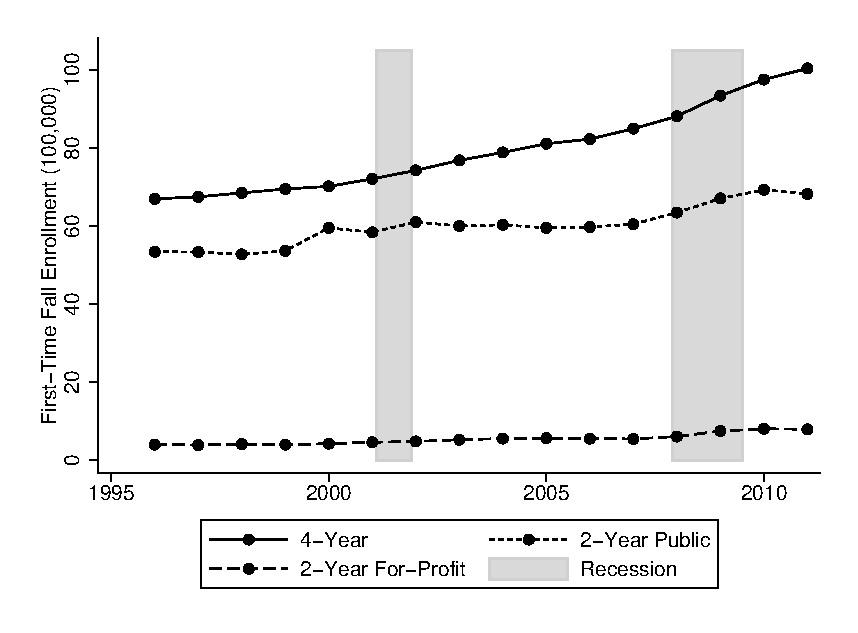
\includegraphics[scale=0.6]{./figures/tef_byyear.eps}&
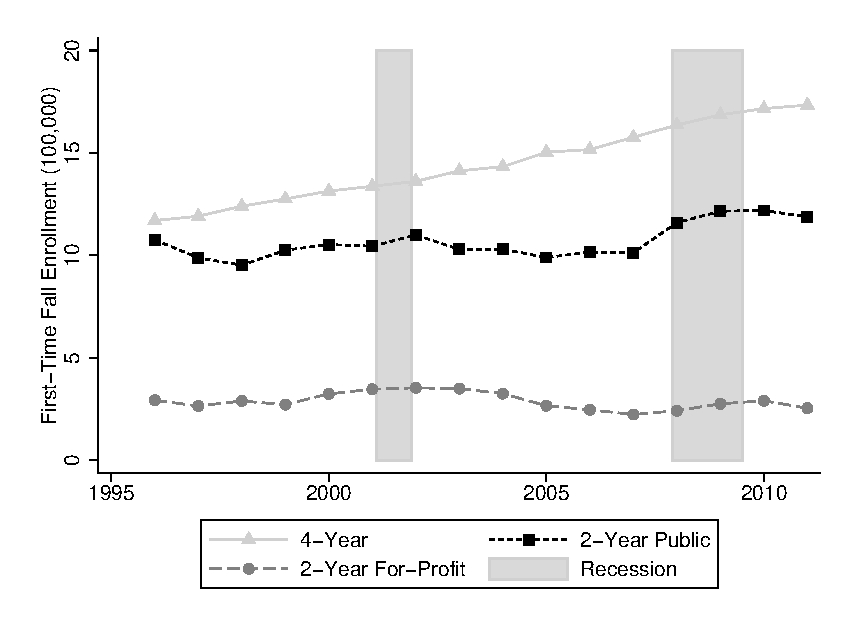
\includegraphics[scale=0.6]{./figures/ffe_byyear.eps}\\
a) Total Enrollment, by Sector&b)First-time Students, by Sector\\

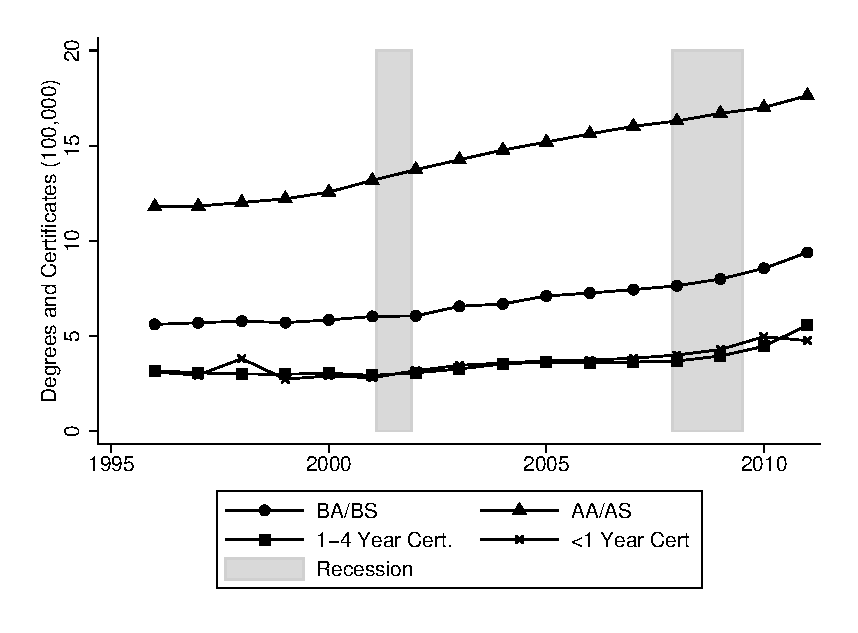
\includegraphics[scale=0.6]{./figures/aw_byyear.eps}&
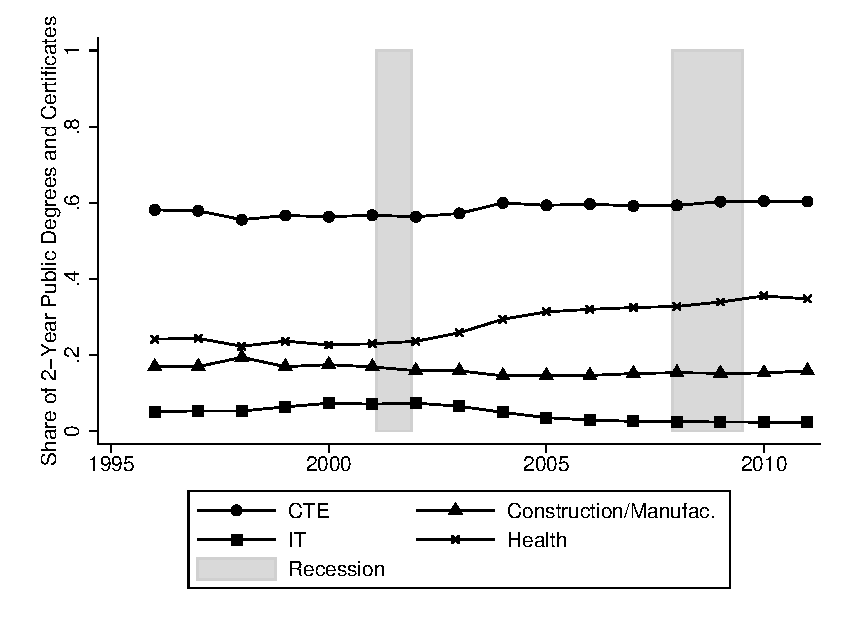
\includegraphics[scale=0.6]{./figures/saw_byyear.eps}\\
c) Total Awards by Type&d) Total 2-Year College Awards by Field\\\\
\multicolumn{2}{p{6in}}{\footnotesize \emph{Notes:} Degree and certificate data is from IPEDS, years 1996-2011. Shaded areas indicate NBER recessions.}
\end{tabular}
\label{fig:grenr}
\end{figure}








\begin{figure}[h]\centering\caption{Enrollment, 2005, Commuting Zones}\begin{tabular}{cc}
\\
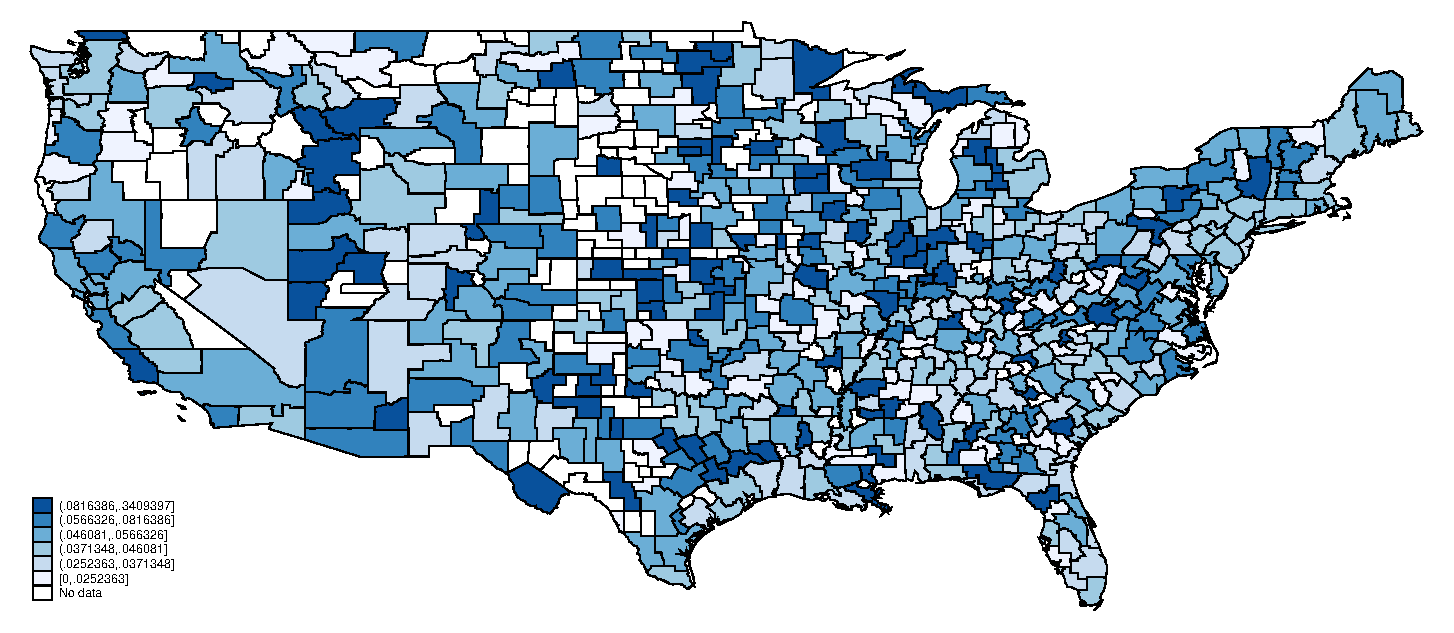
\includegraphics[scale=0.64]{./figures/sh_tef_2005}\\(a) Share of Population in Postsecondary Institutions\\\\
\includegraphics[scale=0.64]{./figures/sh2y_2005}\\
(b) Community College Share of Enrollment\\\\
\multicolumn{2}{p{6in}}{\footnotesize \emph{Notes:} Enrollment data is IPEDS from years 1996-2011, population data is from SEER. Panel (a) displays the share of the population in postsecondary education, while panel (b) displays the share of enrollment accounted for in community colleges.}
\end{tabular}
\label{fig:mapenr}
\end{figure}

\begin{figure}[h]\centering\caption{Content of Community College Awards, 2005, Commuting Zones}\begin{tabular}{cc}
\includegraphics[scale=0.34]{./figures/shaw_CTE_2005}&
\includegraphics[scale=0.34]{./figures/shaw_CON_2005}\\
(a) Share in CTE&(b) Share in Construction/Manufacturing\\
\includegraphics[scale=0.34]{./figures/shaw_HEA_2005}&
\includegraphics[scale=0.34]{./figures/shaw_FAM_2005}\\
(c) Share in Health&(d) Share in Childcare/Cosmetology\\
\multicolumn{2}{p{\textwidth}}{\footnotesize Notes. Figure (a) shows CTE awards as a share of total awards. Figures  (b)-(d) show awards in the particular field as a share of all CTE awards. }\\
\end{tabular}
\label{fig:mapawa}
\end{figure}




\begin{figure}[h]\centering
\caption{Completion Effects and Estimated Earnings Returns }
\begin{tabular}{cc}
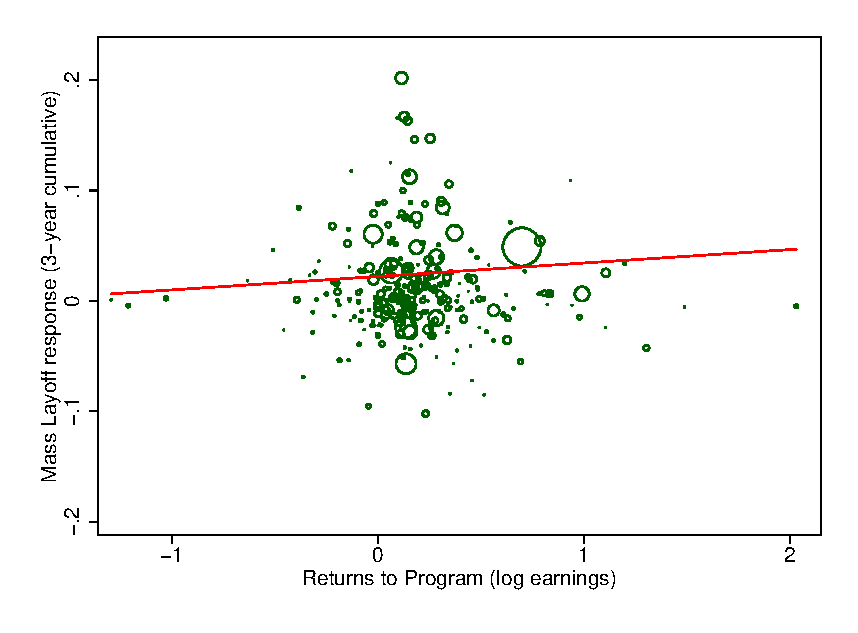
\includegraphics[scale=0.5]{./figures/scatter_bycip_all.eps} &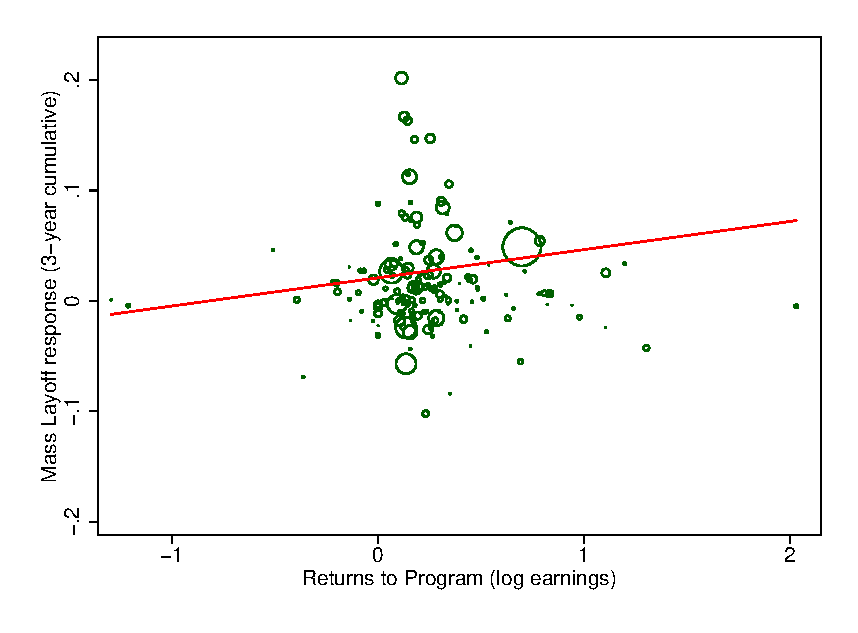
\includegraphics[scale=0.5]{./figures/scatter_bycip_sigret.eps}\\
(a) All Estimates&(b) Statistically Significant Returns Only\\
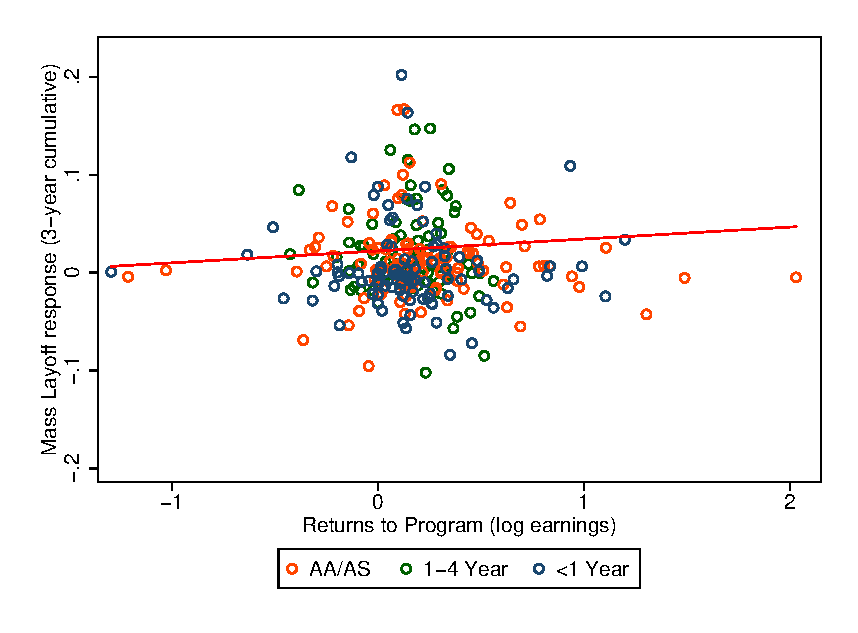
\includegraphics[scale=0.5]{./figures/scatter_bycip_all_bytype.eps} &\includegraphics[scale=0.5]{./figures/scatter_bycip_sigret_bytype.eps}\\
(c) All Estimates&(d) Statistically Significant Returns Only\\\\
\multicolumn{2}{p{\textwidth}}{Notes: Estimated returns from \citet{SKG2014} at the 4-digit Taxonomy of Programs level. Regression line, weighted by the average number of graduates of each program each year, is 0.012 (0.01) in panels a) and c) and 0.026 (0.014) in panels b) and d).}\\
\end{tabular}


\label{fig:scatterallsmall}
\end{figure}




\clearpage

\begin{figure}[h]\centering\caption{Impulse Response Function, Community Colleges, Commuting Zones Level}\begin{tabular}{cc}
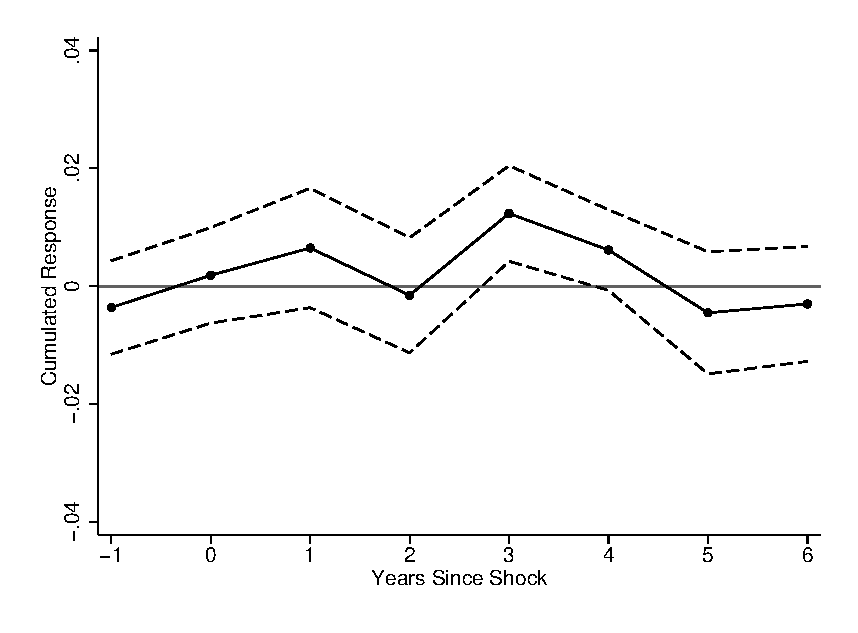
\includegraphics[scale=0.6]{./figures/cumresp_cz_tef_tot47}&
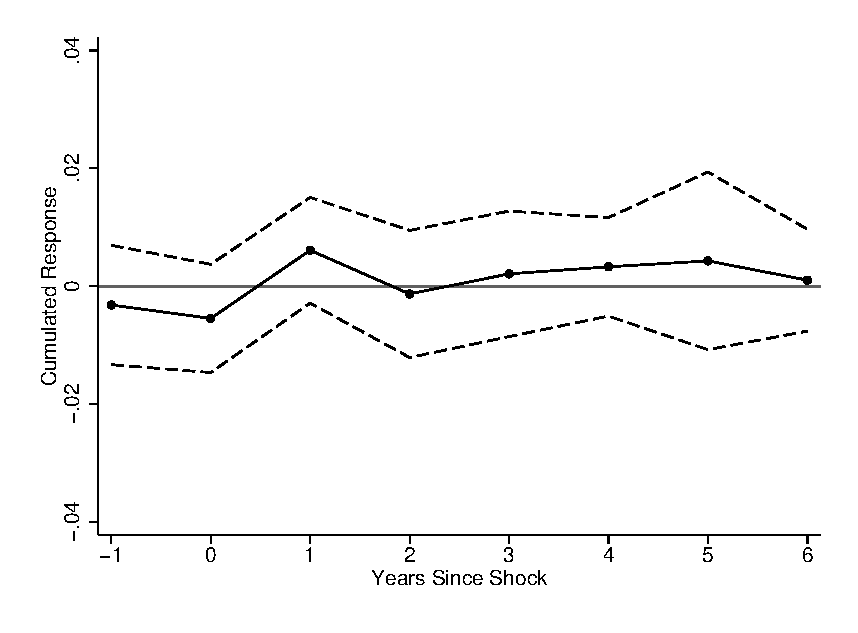
\includegraphics[scale=0.6]{./figures/cumresp_cz_aw_tot47}\\
(a) Fall Enrollment&(b) Total Awards\\
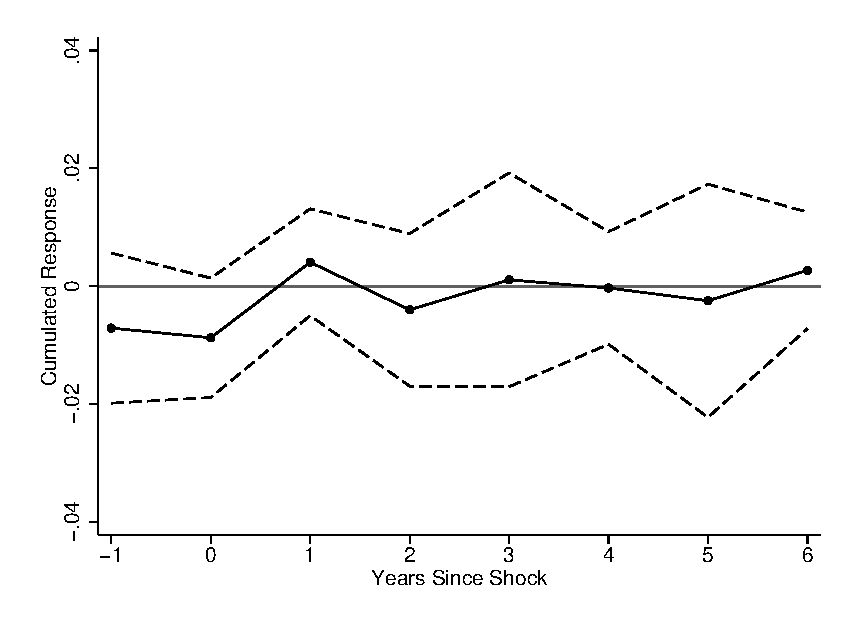
\includegraphics[scale=0.6]{./figures/cumresp_cz_aw_aa47}&
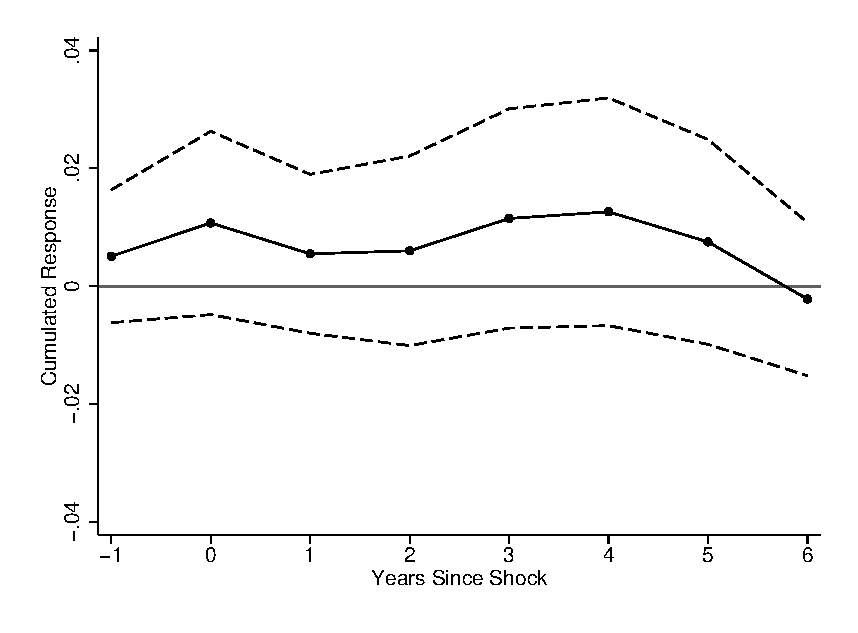
\includegraphics[scale=0.6]{./figures/cumresp_cz_aw_1t447}\\
(c) AA/AS Degrees&(d) 1-4 Year Certificates\\
\multicolumn{2}{p{6in}}{\footnotesize \emph{Notes:} Estimates are from Equation \ref{eqn:localproj}, where the outcome is the panel label. The dotted lines are the 95\% confidence intervals.}
\end{tabular}
\label{fig:czlproj}
\end{figure}



%%%%%%%%%%%%%%%%%%%%%%%%%%%%%%%%%%%%%%%%%%%%%%%%%%%%%%%%%
%Tables
%%%%%%%%%%%%%%%%%%%%%%%%%%%%%%%%%%%%%%%%%%%%%%%%%%%%%%%
\clearpage
\begin{table}[h]\centering\caption{Summary Statistics, 2006-2013}
\def\sym#1{\ifmmode^{#1}\else\(^{#1}\)\fi}\scalebox{0.8}{\begin{tabular}{lc}
\hline\hline

\hline
Workers in Mass Layoffs&   1445.8         \\
                & (6434.5)         \\
Workers in Mass Layoffs as Share of Labor Force&  0.00569         \\
                &(0.00775)         \\
Layoffs $>$ 1\% of Labor Force&    0.203         \\
                &  (0.403)         \\
Layoffs $>$ 5\% of Labor Force&   0.0235         \\
                &  (0.152)         \\
Unemployment Rate&   0.0581         \\
                & (0.0262)         \\
Population (1000s) &    365.7         \\
                & (1047.0)         \\
Population Age 18-60 (1000s) &    206.4         \\
                &  (602.1)         \\
Community Colleges&    2.473         \\
                &  (3.786)         \\
For-Profit 2-year Colleges&    5.294         \\
                &  (16.59)         \\
Community College Fall Enrollment&   9405.8         \\
                &(30857.8)         \\
For-Profit Fall Enrollment&    788.4         \\
                & (2933.5)         \\
No 2-Year Institutions in CZ&   0.0667         \\
                &  (0.250)         \\
Only 2-Year Institutions in CZ&    0.374         \\
                &  (0.484)         \\
Associate's Degrees&   1117.2         \\
                & (2822.0)         \\
1-4 Year Certificates&    559.8         \\
                & (1558.3)         \\
$<$ 1 Year Certificates&    595.8         \\
                & (2027.0)         \\
Share of Awards in CTE&    0.405         \\
                &  (0.174)         \\
Share of Awards in Construction/Manufacturing&   0.0969         \\
                &  (0.110)         \\
Share of Awards in Health&    0.179         \\
                &  (0.118)         \\
Share of Awards in Information Technology&   0.0285         \\
                & (0.0314)         \\
Share of Awards in Public/Protective Services&   0.0380         \\
                & (0.0400)         \\
 
 

\hline\hline
\multicolumn{2}{p{.7\textwidth}}{Notes: Unit of Observation is Commuting Zone by year. Means and standard deviations displayed. }\\
\end{tabular}}
\label{tab:sumstats}
\end{table}







\begin{table}[h]\centering\caption{Mass Layoffs and Two-Year College Enrollment, Degrees and Certificates}
\def\sym#1{\ifmmode^{#1}\else\(^{#1}\)\fi}\scalebox{0.8}{\begin{tabular}{lcccccc}
\hline\hline
&(1)&(2)&(3)&(4)&(5)&(6)\\
&\multicolumn{2}{c}{Fall Enrollment}&\multicolumn{4}{c}{Associate's Degrees and Certificates}\\
&Total&First-Time&Total&AA/AS&1-4 Year Cert& $<$1 Year Cert\\
\hline\\
\multicolumn{4}{l}{\textbf{Community Colleges}}\\
% 
 
Layoffs, t-1    &    0.011         &    0.024\sym{***}&   0.0029         &  -0.0056         &    0.031\sym{*}  &   0.0079         \\
                & (0.0076)         & (0.0092)         & (0.0072)         & (0.0093)         &  (0.017)         &  (0.020)         \\
Layoffs, t-2    &   0.0021         &    0.016\sym{**} &    0.014\sym{**} &   0.0013         &    0.022\sym{**} &    0.038\sym{**} \\
                & (0.0059)         & (0.0071)         & (0.0057)         & (0.0076)         &  (0.011)         &  (0.015)         \\
Layoffs, t-3    &  -0.0017         &   -0.012         &  0.00031         &   -0.018         &    0.022\sym{*}  &    0.012         \\
                & (0.0072)         & (0.0082)         & (0.0054)         &  (0.012)         &  (0.011)         &  (0.015)         \\
 
Total Effect    &    .0111         &    .0287         &     .017         &   -.0227         &    .0741         &    .0584         \\
(se)            &    .0159         &    .0173         &    .0139         &    .0259         &    .0332         &    .0374         \\
P-val           &   0.0000         &   0.0000         &   0.0000         &   0.0000         &   0.0000         &   0.0000         \\
Y-Mean          &  12184.2         &   2138.1         &   1664.7         &   1051.7         &    320.8         &    493.3         \\
Observations    &     6882         &     6882         &     6872         &     6318         &     6714         &     5354         \\
R-sq            &     0.99         &     0.98         &     0.98         &     0.98         &     0.95         &     0.94         \\
 

\\
\hline\\
\multicolumn{4}{l}{\textbf{For-Profits}}\\
% 
 
Layoffs, t-1    &    0.010         &    0.016         &   0.0066         &  -0.0096         &   0.0045         &   0.0045         \\
                & (0.0095)         &  (0.010)         & (0.0085)         &  (0.033)         &  (0.013)         &  (0.021)         \\
Layoffs, t-2    &    0.011         &    0.014         &   0.0071         &   -0.046         &    0.011         &    0.027         \\
                & (0.0088)         & (0.0095)         & (0.0081)         &  (0.029)         &  (0.012)         &  (0.021)         \\
Layoffs, t-3    &    0.012         &    0.011         &    0.025\sym{**} &  -0.0074         &    0.018         &    0.018         \\
                &  (0.011)         &  (0.011)         &  (0.011)         &  (0.033)         &  (0.013)         &  (0.021)         \\
 
Total Effect    &    .0334         &     .041         &    .0386         &   -.0633         &     .034         &    .0499         \\
(se)            &    .0188         &    .0187         &    .0164         &    .0688         &    .0265         &    .0439         \\
P-val           &   0.0000         &   0.0000         &   0.0000         &   0.0000         &   0.0000         &   0.0000         \\
Y-Mean          &   1442.9         &    729.6         &    945.5         &    355.9         &    423.9         &    486.7         \\
Observations    &     4783         &     4783         &     4785         &     2005         &     4656         &     3773         \\
R-sq            &     0.98         &     0.98         &     0.98         &     0.91         &     0.97         &     0.95         \\
 
\\\hline

Year FEs&X&X&X&X&X&X\\
CZ FEs&X&X&X&X&X&X\\
CZ Trends&X&X&X&X&X&X\\
\hline\hline
\multicolumn{7}{p{6in}}{\footnotesize \emph{Notes:} Outcome variables are listed at the top of each column, and are the log counts of the corresponding outcome. Estimates are from equation  \ref{eqn:main}. Panel (a) shows estimates for public community colleges, while panel (b) shows estimates for for-profit schools. All regressions include year and commuting zone fixed effects, commuting zone specific trends. Regressions are weighted by commuting zone population. Standard errors are clustered on commuting zone. *p$<$0.10, ** p$<$0.05, *** p$<$0.01}
\end{tabular}}
\label{tab:main}
\end{table}



\begin{table}[h]\centering\caption{Mass Layoffs and Two-Year College Degrees and Certificates, by Program Type}
\def\sym#1{\ifmmode^{#1}\else\(^{#1}\)\fi}\scalebox{0.8}{\begin{tabular}{lK{2.2cm}K{2.2cm}K{2.2cm}K{2.2cm}K{2.2cm}K{2.2cm}K{2.2cm}}
\hline\hline
&(1)&(2)&(3)&(4)&(5)&(6)&(7)\\
&Total&Career-Technical&Constr./ Manufac.&Health&IT&Public/ Protect.&Childcare/ Cosmet.\\
\hline\\

\multicolumn{6}{l}{\textbf{All Awards}}\\
%\input{../tabfig/lev/reg_mainregawa_ln_aw_tot_47_cz}\hline\\
\multicolumn{6}{l}{\textbf{AA/AS}}\\
%\input{../tabfig/lev/reg_mainregawa_ln_aw_aa_47_cz}\hline\\
\multicolumn{6}{l}{\textbf{1-4 Year Cert}}\\
%\input{../tabfig/lev/reg_mainregawa_ln_aw_1t4_47_cz}\hline\\
\multicolumn{6}{l}{\textbf{$<$1 Year Cert}}\\
%\input{../tabfig/lev/reg_mainregawa_ln_aw_lt1y_47_cz}\\


\hline\hline
\multicolumn{8}{p{7in}}{\footnotesize \emph{Notes:} Estimates are from equation  \ref{eqn:main}. Outcome variables are degrees or certificates awarded in a given field, shown at the column head. Panel (a) shows results for all awards, panel (b) shows results for Associates degrees, panel (c) shows results for longer certificates, and panel (d) shows results for short-term certificate programs. All regressions include year and commuting zone fixed effects, commuting zone specific trends. Regressions are weighted by commuting zone population. Standard errors are clustered on commuting zone. *p$<$0.10, ** p$<$0.05, *** p$<$0.01}
\end{tabular}}
\label{tab:mainbyprog}
\end{table}



\begin{table}[h]\centering\caption{Mass Layoffs and Two-Year College Enrollment, Degrees and Certificates, Before and After 2007}
\def\sym#1{\ifmmode^{#1}\else\(^{#1}\)\fi}\scalebox{0.8}{\begin{tabular}{lcccccc}
\hline\hline
&(1)&(2)&(3)&(4)&(5)&(6)\\
&\multicolumn{2}{c}{Fall Enrollment}&\multicolumn{4}{c}{Degrees and Certificates}\\
&Total&First-Time&Total&AA/AS&1-4 Year Cert& $<$1 Year Cert\\
\hline\\
\multicolumn{4}{l}{\textbf{Community Colleges}}\\
%\input{../tabfig/lev/reg_regprepost_47_cz}
\\
%\hline\\
%\multicolumn{4}{l}{\textbf{For-Profits}}\\
%\input{../tabfig/lev/reg_regprepost_69_cz}\\\hline
Year FEs&X&X&X&X&X&X\\
CZ FEs&X&X&X&X&X&X\\
CZ Trends&X&X&X&X&X&X\\
\hline\hline
\multicolumn{7}{p{6.3in}}{\footnotesize \emph{Notes:} Outcome variables are listed at the top of each column, and are the log counts of the corresponding outcome. Estimates are from equation  \ref{eqn:main}, and allows the effect of mass layoffs to differ before and after 2007. All regressions include year and commuting zone fixed effects, commuting zone specific trends. Regressions are weighted by commuting zone population. Standard errors are clustered on commuting zone. *p$<$0.10, ** p$<$0.05, *** p$<$0.01}
\end{tabular}}
\label{tab:mainrece}
\end{table}



\begin{table}[h]\centering\caption{Mass Layoffs and Two-Year College Enrollment, Degrees and Certificates, Interactions with State-Level Academic Coursework Allowance for UI Beneficiaries}
\def\sym#1{\ifmmode^{#1}\else\(^{#1}\)\fi}\scalebox{0.8}{\begin{tabular}{lccccc}
\hline\hline
&(1)&(2)&(3)&(4)&(5)\\
&\multicolumn{2}{c}{Fall Enrollment}&\multicolumn{3}{c}{Degrees and Certificates}\\
&Total&First-Time&Total&CTE&Academic\\
\hline\\

%\input{../tabfig/lev/reg_reguiaca_47_cz}
\\
%\hline\\
%\multicolumn{4}{l}{\textbf{For-Profits}}\\
%\input{../tabfig/lev/reg_regprepost_69_cz}\\\hline
Year FEs&X&X&X&X&X\\
CZ FEs&X&X&X&X&X\\
CZ Trends&X&X&X&X&X\\
\hline\hline
\multicolumn{6}{p{6.01in}}{\footnotesize \emph{Notes:} Outcome variables are listed at the top of each column, and are the log counts of the corresponding outcome. Estimates are from equation  \ref{eqn:main}, and allows the effect of mass layoffs to differ by whether the state allowed UI beneficiaries to enroll in academic coursework without losing benefits, as in Figure 2 of \citet{BT2015}. All regressions include year and commuting zone fixed effects, commuting zone specific trends. Regressions are weighted by commuting zone population. Standard errors are clustered on commuting zone. *p$<$0.10, ** p$<$0.05, *** p$<$0.01}
\end{tabular}}
\label{tab:mainuibt}
\end{table}





\begin{table}[h]\centering
\caption{Distribution of T-Statistics from Alternate Commuting Zone Definitions}\scalebox{0.8}{
\begin{tabular}{lcccccc}
\hline\hline
&(1)&(2)&(3)&(4)&(5)&(6)\\
&\multicolumn{2}{c}{Fall Enrollment}&\multicolumn{4}{c}{Associate's Degrees and Certificates}\\
&Total&First-Time&Total&AA/AS&1-4 Year Cert& $<$1 Year Cert\\\hline\\
{Layoffs, t-1} &[1.21, 2.20]     & [2.11, 3.06]&[-0.35, 1.11] &[-2.23, -0.45]&[0.967, 1.95]&[0.08, 1.43]\\
{Layoffs, t-2} &[1.14, 2.39]     & [2.91, 4.06] &[1.96, 3.39]&[-0.004, 1.48]&[1.01, 2.57]&[0.94, 2.64]\\
{Layoffs, t-3}& [-1.04, -0.22]     & [-1.82, -0.72] &[-0.29, 1.07]&[-1.53, 0.22]&[1.30, 2.42]&[-0.49, 1.46]\\
\hline\hline
\multicolumn{7}{p{6in}}{\footnotesize \emph{Notes:} Results shown from the test outlined in \citet{FKV2017}, and discussed in Section \ref{sec:robchecks}. The row for each coefficient shows the 2.5th and 97.5th percentile of the distribution of t-statistics on the noted coefficient, when running the analysis with each of  1000 different commuting zone realizations.}
\end{tabular}}
\label{tab:FKVtest}
\end{table}


%
%\begin{table}[h]\centering\caption{Mass Layoffs and Two-Year College Enrollment, Degrees and Certificates, by UI approval}
%\def\sym#1{\ifmmode^{#1}\else\(^{#1}\)\fi}\scalebox{0.8}{\begin{tabular}{lcccccc}
%\hline\hline
%&(1)&(2)&(3)&(4)&(5)&(6)\\
%&\multicolumn{2}{c}{Fall Enrollment}&\multicolumn{4}{c}{Degrees and Certificates}\\
%&Total&First-Time&Total&AA/AS&1-4 Year Cert& $<$1 Year Cert\\
%\hline\\
%\multicolumn{4}{l}{\textbf{Community Colleges}}\\
%\input{../tabfig/lev/reg_reguiaca_47_cz}
%\\
%%\hline\\
%%\multicolumn{4}{l}{\textbf{For-Profits}}\\
%%\input{../tabfig/lev/reg_regprepost_69_cz}\\\hline
%Year FEs&X&X&X&X&X&X\\
%CZ FEs&X&X&X&X&X&X\\
%CZ Trends&X&X&X&X&X&X\\
%\hline\hline
%\end{tabular}}
%\label{tab:mainui}
%\end{table}



\clearpage
\appendix
\section{Appendix Tables and Figures}
\label{subsec:apptab}
\setcounter{table}{0}
\renewcommand{\thetable}{A\arabic{table}}   
\setcounter{figure}{0}
\renewcommand{\thefigure}{A\arabic{figure}}   


\end{document}
